\documentclass{article}
\usepackage{graphicx}

\title{CS 181 Report for Programming Assignment 1}
\author{Rajan Saini}
\begin{document}
\maketitle
\section{Methodology}
For this assignment, we were tasked with perspective-shifting two images of the same
object. I used python 3, with opencv and numpy to do the rendering and computation.
\begin{enumerate}
\item A set of points common to both images were identified and labeled, using the 
      OpenCV library in Python to take care of I/O. I assigned each point a
      different color along a blue-green gradient so that common points can be
      better identified by a human.
\item The homography problem was solved manually in get\_H(). I set up a system
of equations encoded by matrices A and B, and used numpy's lstsq function to find the
solution of minimal norm. This was necessary because the number of equations 
exceeded the number of variables. 
\item The homography matrix was then used to transform one image to match the
perspective of the other, using OpenCV's warpPerspective. An interesting
artifact is that the transformation also warps the labels. I chose to keep that
the skewed labels because they visually illustrate the effects and shortcomings of the
perspective-shifting.
\end{enumerate}
\section {Results}
\subsection {Building at UCSB}
Points on the left image:
[(360, 353), (534, 336), (1270, 450), (1279, 608), (1330, 710), (537, 526)]
Points on the right image:
[(189, 610), (317, 556), (1192, 428), (1190, 636), (1280, 755), (313, 729)]
H matrix when transforming left to match right:
[[ 5.17213949e-01  4.46050703e-02 -2.27947002e+01]
 [-4.09746925e-01  7.92448909e-01  4.07924600e+02]
 [-3.63547094e-04  6.92570923e-05  1.00000000e+00]]
H matrix when transforming right to match left:
[[ 1.89031295e+00  1.21536422e-01 -1.11487360e+01]
 [ 6.62536716e-01  1.43342651e+00 -5.83816082e+02]
 [ 6.68941110e-04  5.48086805e-05  1.00000000e+00]]
\begin{itemize}
\item I used the given images on GauchoSpace for this part.
\end{itemize}
Left original
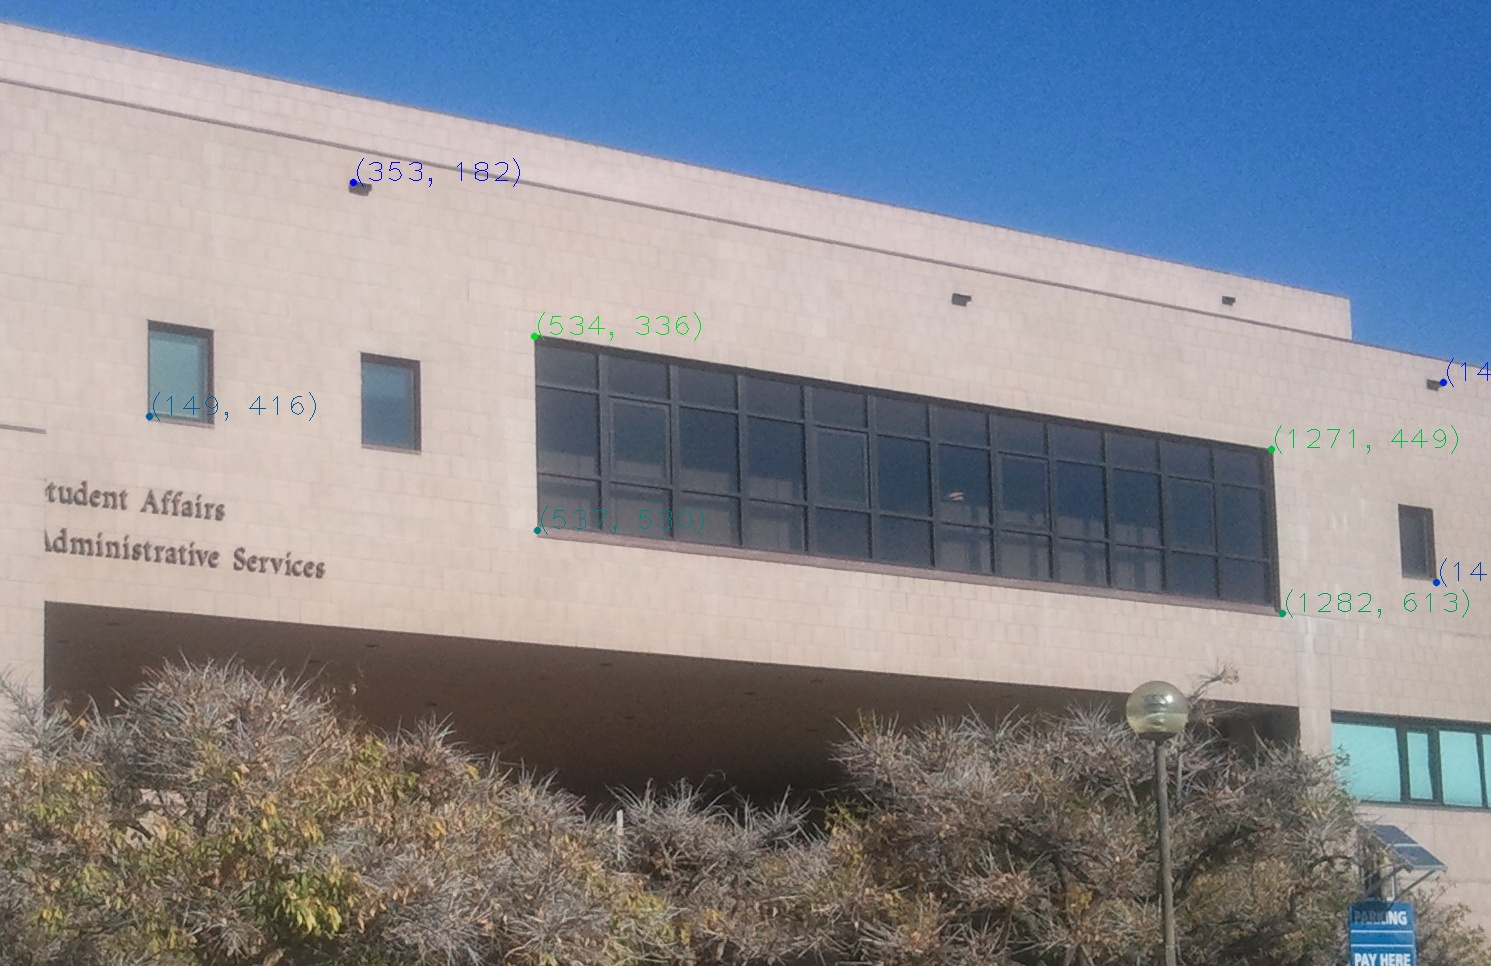
\includegraphics[width=\linewidth]{./results/building/left.jpg}
Right original
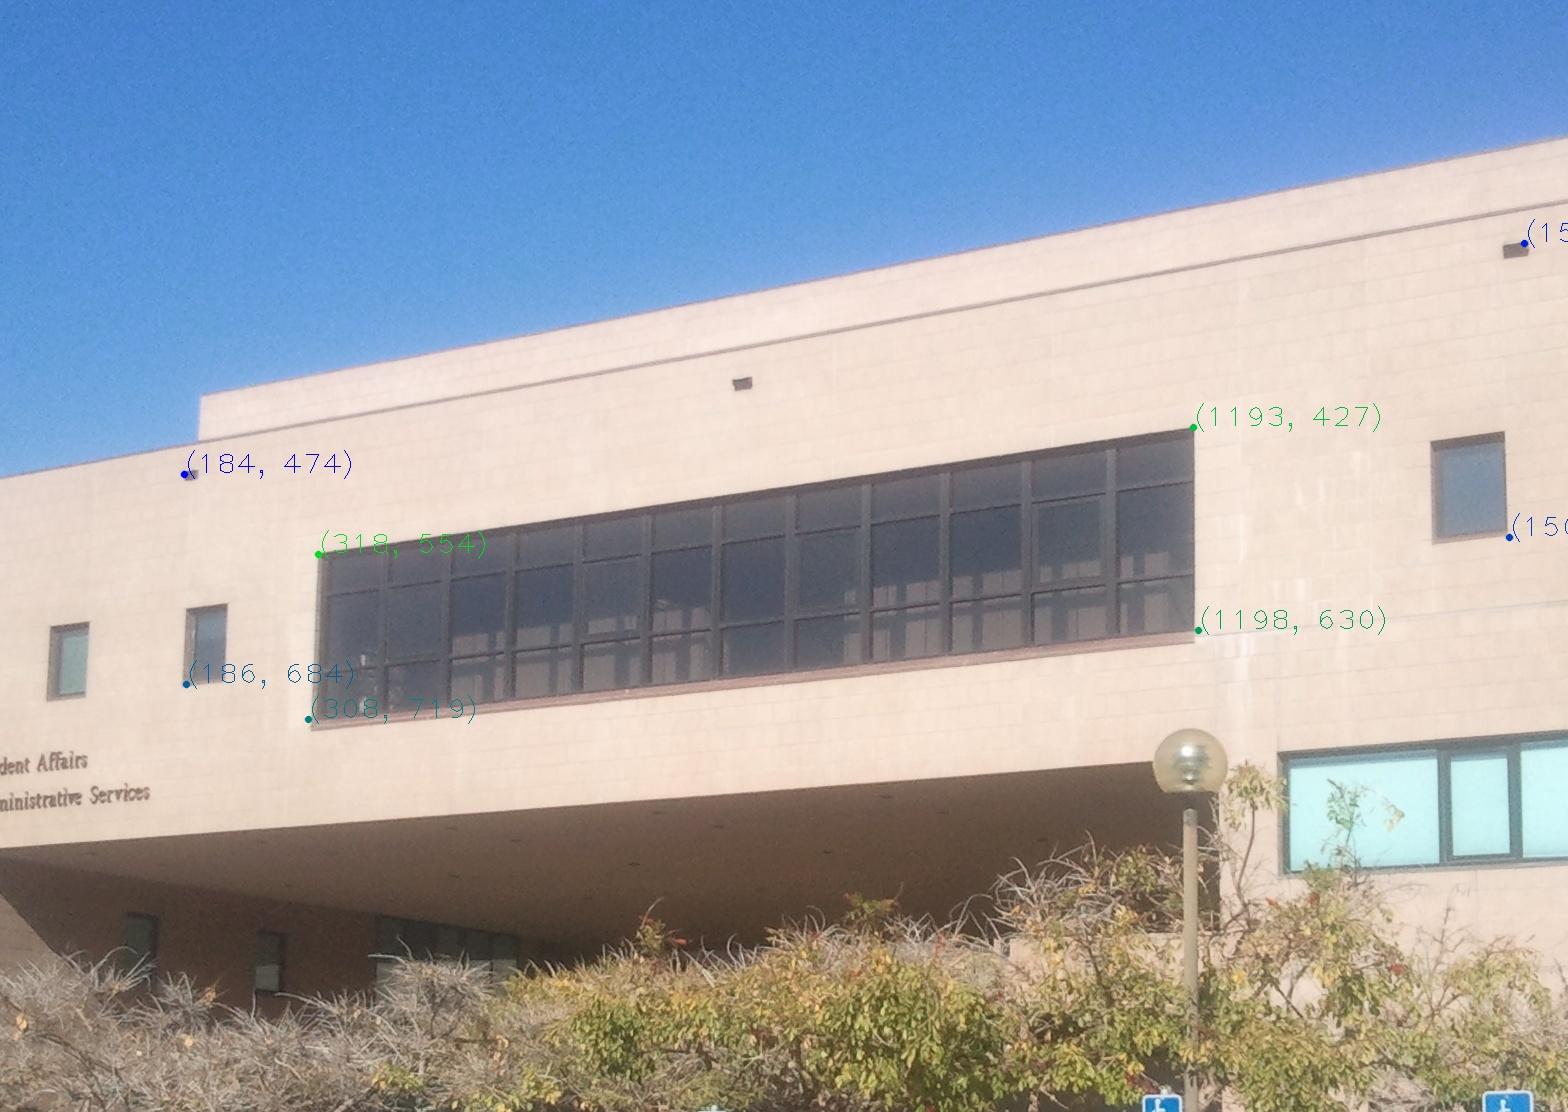
\includegraphics[width=\linewidth]{./results/building/right.jpg}
Left transformed to right 
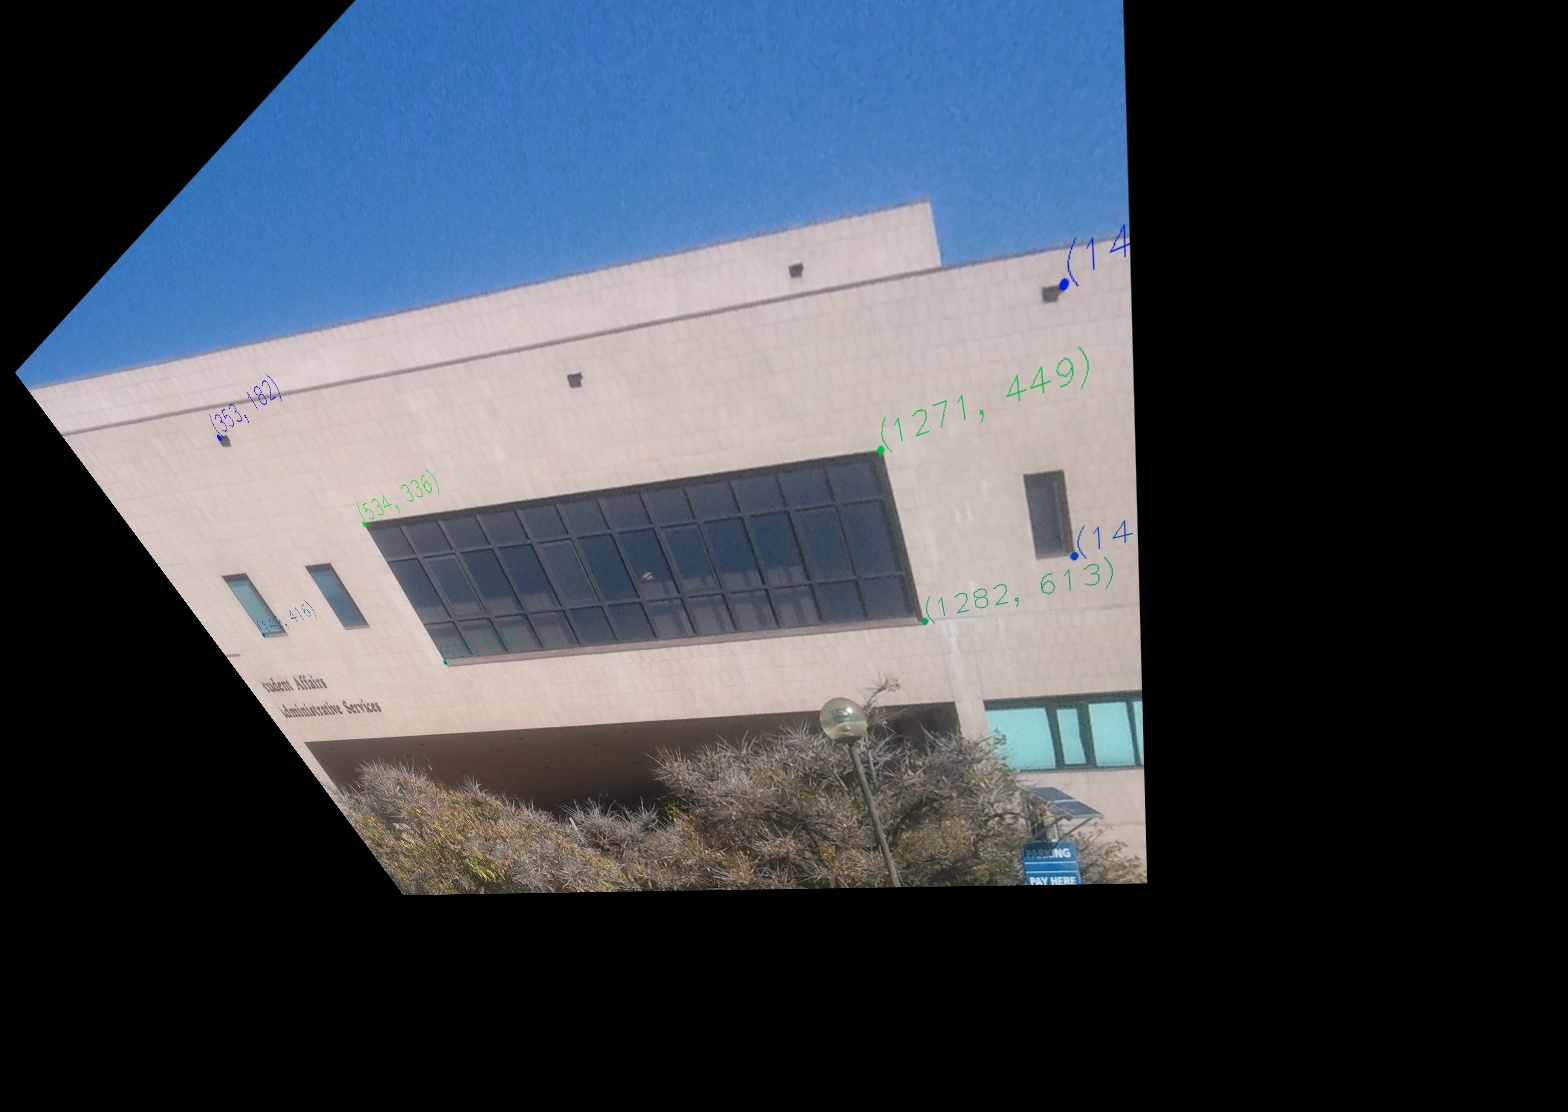
\includegraphics[width=\linewidth]{./results/building/left_transformed.jpg}
Right transformed to left
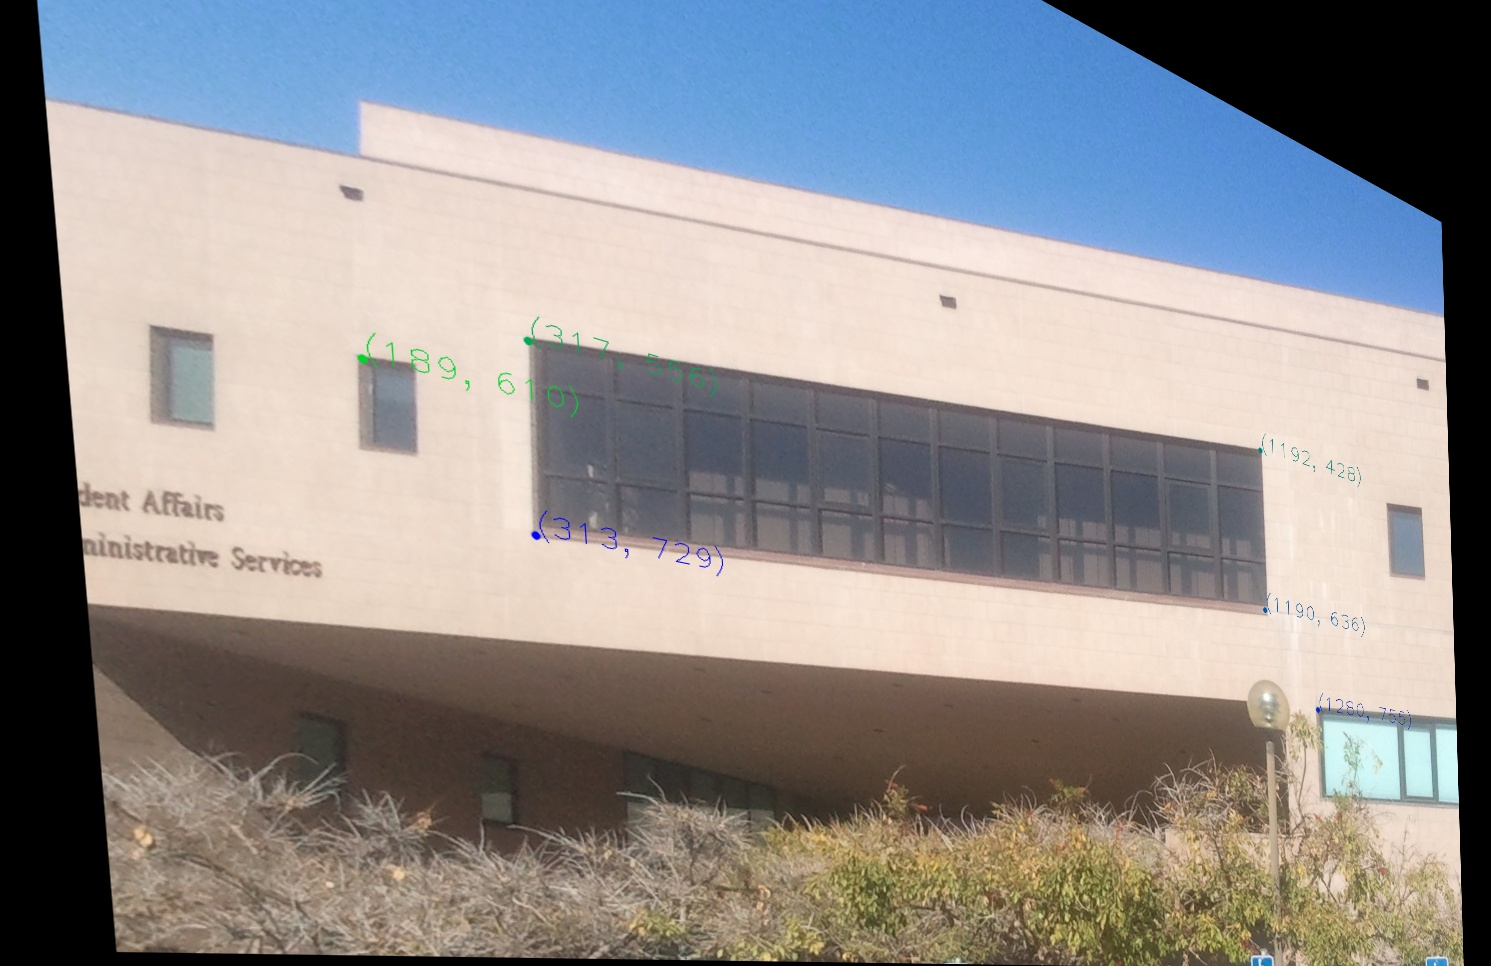
\includegraphics[width=\linewidth]{./results/building/right_transformed.jpg}
\subsection {Voices of Fire Painting}
Points on the left image:
[(111, 41), (147, 41), (148, 120), (110, 121)]
Points on the right image:
[(284, 102), (482, 139), (494, 602), (279, 621)]
H matrix when transforming left to match right:
[[ 1.03756256e+01  2.46860072e+00 -8.20039118e+02]
 [ 2.13031357e+00  1.00643095e+01 -4.93141013e+02]
 [ 4.35641405e-03  2.75857441e-03  1.00000000e+00]]
H matrix when transforming right to match left:
[[ 6.61115198e-02  3.64662373e-02  7.20229606e+01]
 [-7.14122458e-02  3.24562974e-01  2.44761202e+01]
 [-5.58597259e-04  2.69585950e-04  1.00000000e+00]]
Far original 
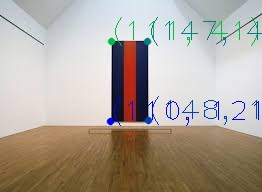
\includegraphics[width=\linewidth]{./results/voices_of_fire/far.jpg}
Side original
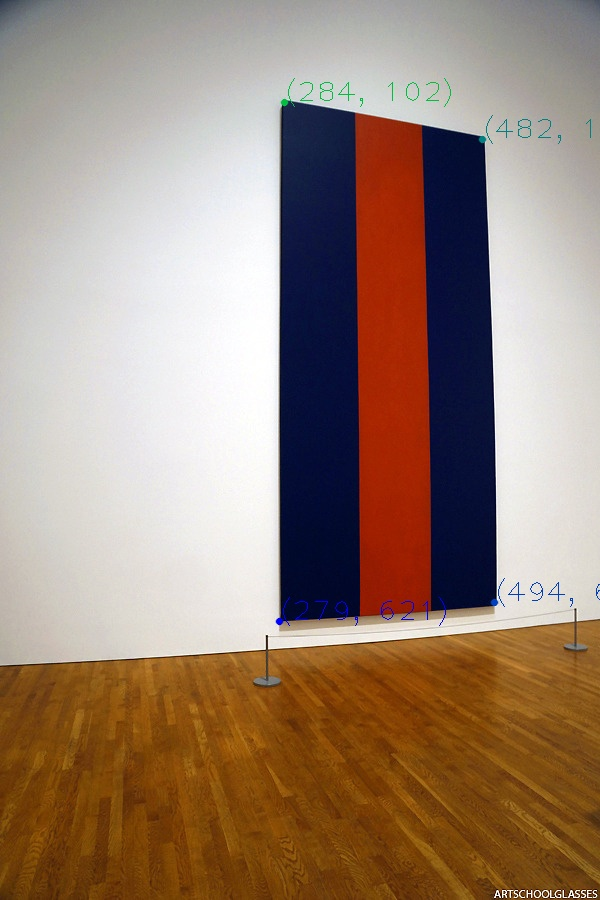
\includegraphics[width=\linewidth]{./results/voices_of_fire/side.jpg}
Far transformed to side

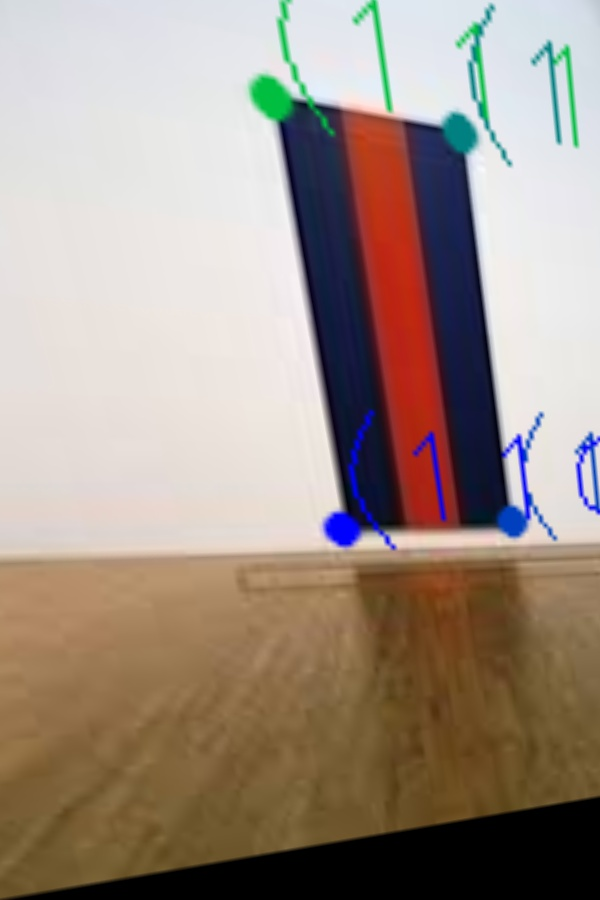
\includegraphics[width=\linewidth]{./results/voices_of_fire/far_transformed.jpg}
Side transformed to far
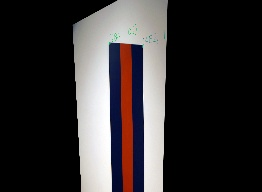
\includegraphics[width=\linewidth]{./results/voices_of_fire/side_transformed.jpg}

\section{Code}
Code can be found at https://github.com/rajansaini691/homography
\end{document}

